\documentclass[letter,12pt]{article}
\usepackage{epsfig,latexsym,amsmath,amssymb,epic,eepic,psfrag,subfigure,float,euscript,array}
\usepackage[latin1]{inputenc}
\usepackage{standalone}
\usepackage{tikz,pgf,pgfplots}
\usepackage[margin=2.5cm]{geometry}

\newenvironment{exercise}[1][Uppgift]{\begin{trivlist} \item[\hskip
    \labelsep {\stepcounter{exerctr}\bfseries #1
      \arabic{exerctr}}]}{\end{trivlist}\vspace{10mm}}

\newcounter{exerctr}
\newcounter{abcctr}[exerctr]

\newcommand{\abc}{\noindent\vspace{1mm}\\ {\bf
    \stepcounter{abcctr}(\alph{abcctr})\ }}
\newcommand{\bbm}{\begin{bmatrix}}
\newcommand{\ebm}{\end{bmatrix}}
\newcommand{\point}[1]{\hfill {\bf (#1p)}\\ \vspace{-5mm}}
\newcommand{\ctrb}{\EuScript{S}}
\newcommand{\Lap}{\mathcal{L}}
\newcommand{\obsv}{\EuScript{O}}
\newcommand{\realdel}[1]{\text{Re}\left\{#1\right\}}
\newcommand{\imagdel}{\text{Im}}
\newcommand{\bC}{\mathbb{C}}
\newcommand{\bR}{\mathbb{R}}
\newcommand{\bmpv}{\begin{minipage}[t]}
\newcommand{\bmps}{\begin{minipage}[t]{45mm}}
\newcommand{\bmpm}{\begin{minipage}[t]{90mm}}
\newcommand{\bmpl}{\begin{minipage}[t]{\textwidth}}
\newcommand{\emp}{\end{minipage}}
\newcommand*{\zethree}{\big(z - \mexp{-3h}\big)}
\newcommand*{\mexp}[1]{\ensuremath{\mathrm{e}^{#1}}}

\newcommand*\circled[1]{\tikz[baseline=(char.base)]{
            \node[shape=circle,draw,inner sep=2pt] (char) {#1};}}

\addtolength{\topmargin}{-1cm}
\textheight 23.5cm
%\oddsidemargin 0.61cm
%\evensidemargin 0.61cm


\def\OctaveG{tf([0.5 1], [1 0 -1])}

\title{Computerized control partial exam 2 (15\%)}
\author{Kjartan Halvorsen}

\begin{document}

\maketitle


\begin{description}
\item[Time] 2016-10-28 17:35 - 19:00
\item[Place] 4101
\item[Permitted aids] The single colored page with your own notes, table of Laplace transforms, calculator
\end{description}

All answers should be readable and well motivated (if nothing else is written). Solutions/motivations should be written on the provided spaces in this exam. Use the last page if more space is needed.

\begin{center}
{\Large Good luck!} \\
\end{center}

\noindent
\fbox{
\bmpl
{\bf Matricual and name:}\\
\vspace*{30mm}
\emp}

\clearpage

%-----------------------------------------------------------------


\subsection*{Problem 1 (60p)}

\subsubsection*{(a) 40p}
The plant in figure \ref{fig:2dof} is described by the pulse-transfer function
\begin{equation}
H(z) = \frac{1}{z-0.9}.
\end{equation}
The specifications on the closed-loop system is that the closed loop system from the command signal to the output should be 
\begin{equation}
H_c(z) = \frac{0.5}{z-0.5},
\end{equation}
that all observer poles should be placed in the origin, and that the steady-state error for constant disturbances $d$ should be eliminated. 

Determine the polynomials \(R(z)\), \(S(z)\) and \(T(z)\) in an RST controller of the form in figure~\ref{fig:2dof}, such that the specifications are satisfied.

\begin{figure}
\begin{center}
\includegraphics[width=0.7\linewidth]{../../homework/rst-block}
\caption{RST controller}
\label{fig:2dof}
\end{center}
\end{figure}

\noindent
\fbox{
\bmpl
{\bf Controller design:}\\
\vspace*{80mm}
\emp}

\noindent
\fbox{
\bmpl
{\bf Controller design, contd:}\\
\vspace*{100mm}
\emp}


\subsubsection*{(b) 20p}

Determine the closed-loop pulse transfer function $H_{d}(z)$ from the disturbance $d$ to the output $y$, and show that with the controller from problem (a), constant disturbances are eliminated, i.e.~that $H_d(1) = 0$. 

\noindent
\fbox{
\bmpl
{\bf Solution:}\\
\vspace*{80mm}
\emp}


\clearpage
\subsection*{Problem 2 (40p)}
Assume, now, that the plant \(H(z) = \frac{1}{z-0.9}\) is controlled by feedback from the control error, as illustrated in figure~\ref{fig:feedback}, using the controller
\[ F(z) = K\frac{z}{z-1}. \]

\begin{figure}
\begin{center}
     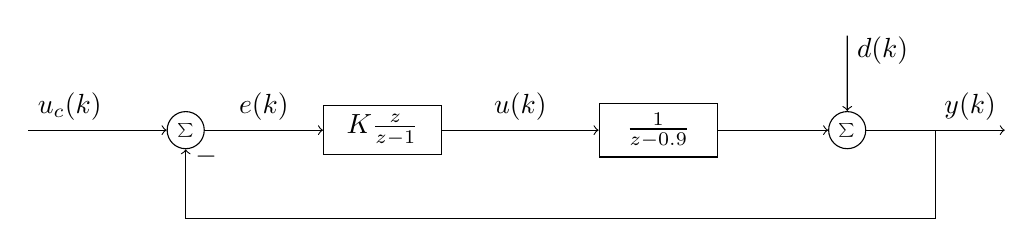
\begin{tikzpicture}[scale = 0.8, node distance=25mm, block/.style={rectangle, draw, minimum width=15mm}, sumnode/.style={circle, draw, inner sep=2pt}]
     
     \node[coordinate] (refinput) {};
     \node[sumnode, right of=refinput, node distance=20mm] (sumerr) {\tiny $\sum$};
     \node[block, right of=sumerr] (controller) {$K\frac{z}{z-1}$};
     %\node[above of=controller, node distance=6mm] {controller};
     \node[block, right of=controller, node distance=35mm] (plant) {$\frac{1}{z-0.9}$};
     \node[sumnode, right of=plant, node distance=24mm] (sum) {\tiny $\sum$};
     %\node[above of=tank, node distance=6mm] {motor};
     \node[coordinate, right of=sum, node distance=20mm] (output) {};
     \node[coordinate, above of=sum, node distance=12mm] (disturbance) {};

     \draw[->] (refinput) -- node[above, pos=0.3] {$u_c(k)$} (sumerr);
     \draw[->] (sumerr) -- node[above] {$e(k)$} (controller);
     \draw[->] (controller) -- node[above] {$u(k)$} (plant);
     \draw[->] (plant) -- (sum);
     \draw[->] (sum) -- node [coordinate] (measure)  {} node [above, near end] {$y(k)$} (output);
     \draw[->] (disturbance) -- node[right, pos=0.2] {$d(k)$} (sum);
     \draw[->] (measure) -- ++(0,-14mm) -| node[right, pos=0.95] {$-$} (sumerr);
     \end{tikzpicture}
     \caption{Feedback control from the error signal.}
     \label{fig:feedback}
   \end{center}
 \end{figure}
 
\subsubsection*{(a) 20p}

Figure~\ref{fig:rlocus} shows the root locus for the closed-loop poles with respect to the gain $K$. In figure~\ref{fig:step}, four different step plots are shown for four different values of $K$. Identify (and circle) the corresponding step plot for each value of $K$ in the table below.

\begin{center}
\begin{tabular}{cl}
\(K\) & Step plot\\\hline
0.002 & A\hspace*{2mm} B\hspace*{2mm} C\hspace*{2mm} D\\
1.0 & A\hspace*{2mm}  B\hspace*{2mm}  C\hspace*{2mm} D\\
3.0 & A\hspace*{2mm} B\hspace*{2mm}  C\hspace*{2mm} D\\
4.0 & A\hspace*{2mm} B\hspace*{2mm}  C\hspace*{2mm} D\\ \hline
\end{tabular}
\end{center}

\begin{figure}[bp]
\begin{center}
\begin{tikzpicture}
    \node[anchor=south west,inner sep=0] at (0,0) {\includegraphics[width=0.5\linewidth]{p2_rlocus_rlocus-crop}};
    \node[coordinate, pin={[pin distance=20mm] 80:{$K=0.003$}}] at (7.17,3.47) {};
    \node[coordinate, pin={[pin distance=20mm] 115:{$K=3.8$}}] at (3.77,3.47) {};
\end{tikzpicture} 

\caption{Root locus wrt the gain $K$.}
\label{fig:rlocus}
\end{center}
\end{figure}

\begin{figure}[tp]
\begin{center}
\begin{tabular}{cc}
A & B\\
\includegraphics[width=0.4\linewidth]{step-plot-3-crop}
&\includegraphics[width=0.4\linewidth]{step-plot-1-crop}\\
C & D\\
\includegraphics[width=0.4\linewidth]{step-plot-5-crop}
&\includegraphics[width=0.4\linewidth]{step-plot-2-crop}

\end{tabular}
\caption{Step responses for different values of $K$.}
\label{fig:step}
\end{center}
\end{figure}

\clearpage
\subsubsection*{(b) 20p}

Determine the gain $K$ so that the closed loop system has poles with realpart equal to $0.7$.


\noindent
\fbox{
\bmpl
{\bf Solution:}\\
\vspace*{150mm}
\emp}

\cleardoublepage

\noindent
{\bf If necessary,} you can continue your solutions on this sheet. Mark clearly which problem the solution corresponds to.

%\end{document}

\section*{Solutions}
\subsection*{Problem 1}

\subsubsection*{(a)}
Since we have the requirement that constant disturbances on the output must be eliminated, then the loop gain must contain at least one integrator. The plant itself does not have an integrator, so this must be provided by the controller \(\frac{S(z)}{R(z)}\). We must thus have the feedback controller
\[\frac{S(z)}{(z-1)\bar{R}(z)},\] which has \(2n_{\bar{R}} + 2\) unknown coefficients. These coefficients are to be determined from the Diophantine equation
\[ A(z)(z-1)\bar{R}(z) + B(z)S(z) = A_{cl}(z), \] from which we obtain \(n_{\bar{R}} + 2\) equations in the coefficients. The degree of the \(\bar{R}\) polynomial must have degree \(n_{\bar{R}} = 0\), i.e the feedback controller is 
\[ \frac{s_0z + s_1}{z-1}. \]

The left hand side of the Diophantine equation is of degree 2, so on the right hand side we have \(A_c(z) = z-0.5\) and \(A_o(z) = z\). We can now set up the Diophantine equation
\[ (z-0.9)(z-1) + s_0z + s_1 = z^2 - 0.5z \]
from which we get
\[ s_1 = -0.9 \qquad s_0 = -0.5+1.9 = 1.4\]

The closed-loop system becomes
\[ H_c(z) = \frac{T(z)B(z)}{A(z)R(z) + B(z)S(z)} =   \frac{T(z)B(z)}{A_c(z)A_o(z)} \]
which we set equal to the desired closed-loop system
\[  \frac{T(z)B(z)}{A_c(z)A_o(z)}  = \frac{B_c(z)}{A_c(z)},\] and get
\[ T(z) = \frac{A_o(z)B_c(z)}{B(z)} = 0.5z. \]

The controller is thus
\begin{align*}
H_{fb}(z) &= \frac{S(z)}{(z-1)\bar{R}(z)} = \frac{1.4z - 0.9}{z-1}\\
H_{ff}(z) &= \frac{T(z)}{(z-1)\bar{R}(z)} = \frac{0.5z}{z-1}. 
\end{align*}

\subsubsection*{(b)}
Using Mason's rule:
\begin{equation*}
\begin{split}
 H_d(z) &= \frac{1}{1 + \frac{B}{A}\cdot\frac{S}{R}} = \frac{A(z)R(z)}{A(z)R(z) + B(z)S(z)} \\
        &= \frac{A(z)R(z)}{A_c(z)A_o(z)} = \frac{(z-0.9)(z-1)}{(z-0.5)z}. 
      \end{split}
\end{equation*}

Wee se directly that
\[ H_d(1) = \frac{(1-0.9)(1-1)}{(1-0.5)1} = 0. \]

\subsection*{Problem 2}

\subsubsection*{(a)}

The root locus starts with two poles at $1$ and $0.9$. For small values of $K$ we will have poles that are slow and completely damped. The only such response is \textbf{B}. As $K$ increases we will have closed-loop poles that follows the unit circle a bit inside it. The poles will have little damping and will increase in speed with $K$. Finally, one pole move outside the unit circle, and the system becomes unstable. With this motivation it is clear that we get

\begin{center}
\begin{tabular}{cl}
\(K\) & Step plot\\\hline
0.002 & A\hspace*{2mm} \circled{B}\hspace*{2mm} C\hspace*{2mm} D\\
1.0 & A\hspace*{2mm}  B\hspace*{2mm}  C\hspace*{2mm} \circled{D}\\
3.0 & \circled{A}\hspace*{2mm} B\hspace*{2mm}  C\hspace*{2mm} D\\
4.0 & A\hspace*{2mm} B\hspace*{2mm}  \circled{C}\hspace*{2mm} D\\ \hline
\end{tabular}
\end{center}

\subsubsection*{(b)}

The closed-loop system from command signal to the output is
\[ H_c(z) = \frac{K \frac{z}{z-1}\frac{1}{z-0.9}}{1 + K \frac{z}{z-1}\frac{1}{z-0.9}} = \frac{Kz}{(z-1)(z-0.9) + Kz}. \]
The characteristic equation is 
\[ (z-1)(z-0.9) + Kz = z^2 - (1.9-K)z + 0.9 = 0 \]
with solution
\[ z = \frac{1.9-K}{2} \pm \frac{1}{2}\sqrt{(1.9-K)^2 - 5.6}. \]
We know from the root locus that for a value of  $K$ that gives poles with real part $0.7$, then the poles are complex-conjugated and so the expression under the root sign must be negative. The real part is given by the first term in the solution to the quadratic equation. We get
\[ \frac{1.9-K}{2} = 0.7 \quad \Rightarrow \quad K = 1.9-1.4 = 0.5 \]

\end{document}
